\documentclass[a4paper,12pt]{article}

\usepackage[utf8]{inputenc}
\usepackage{graphicx}
\usepackage{float}

\title{WeScrabble\\ \small Project for the course: Distributed and Mobile Programming Paradigm}
\author{Titouan Christophe}
\date{\today}

\begin{document}
\maketitle

\section{The game}
\begin{figure}[H]
  \center
  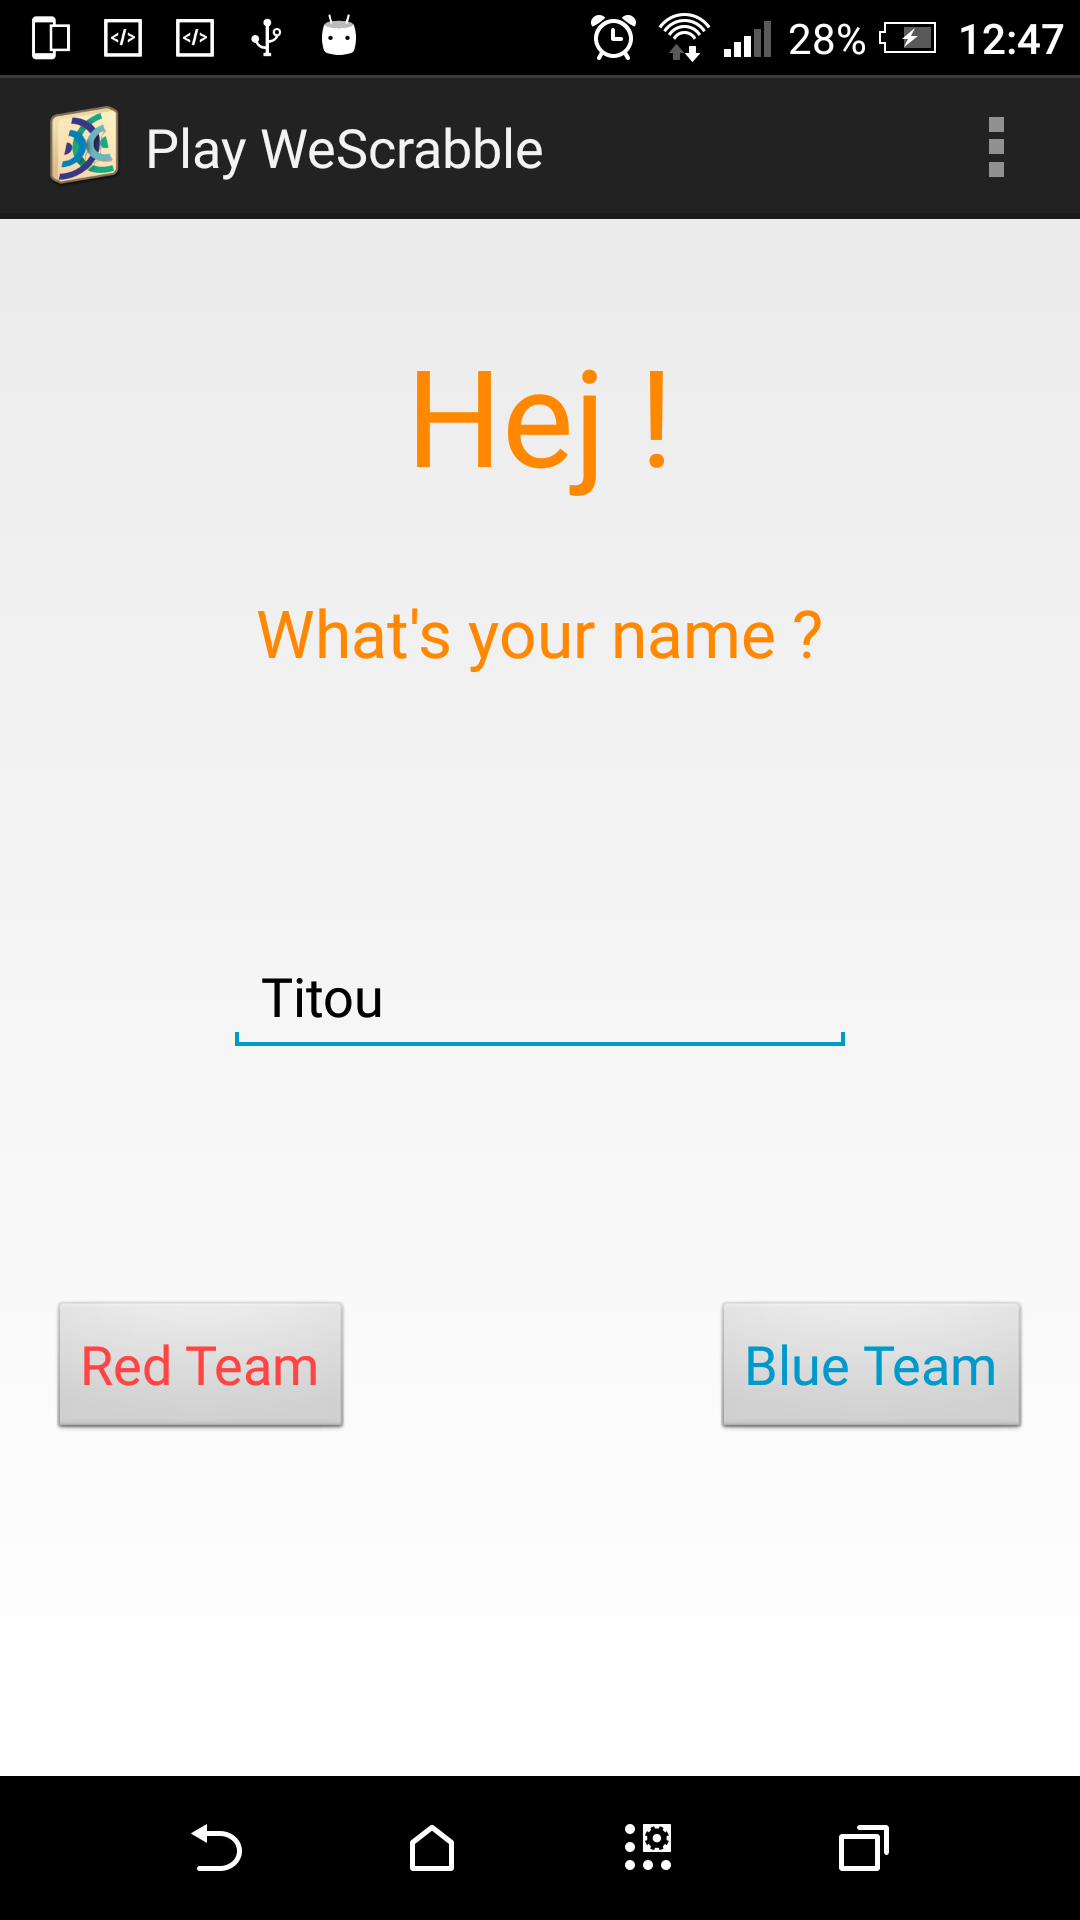
\includegraphics[width=.32\textwidth]{login.png}\hfill
  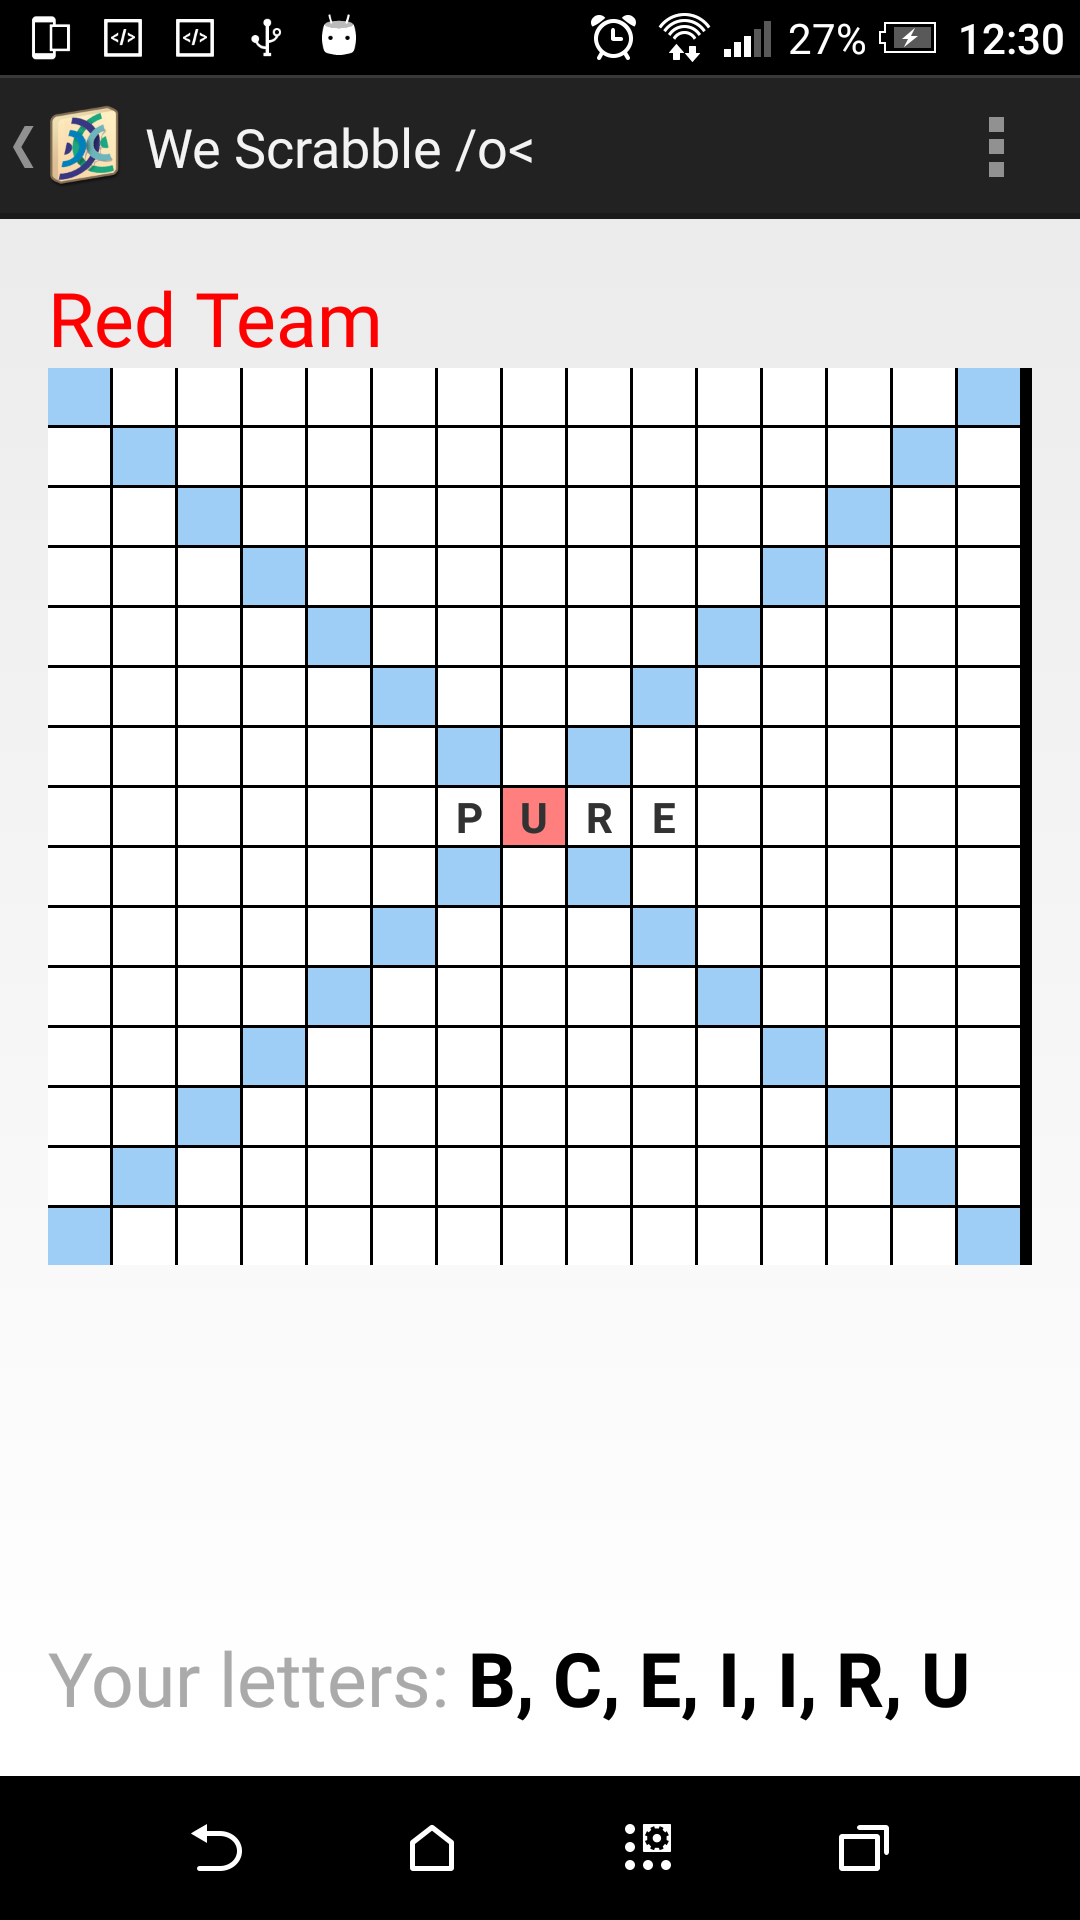
\includegraphics[width=.32\textwidth]{screenshot.png}\hfill
  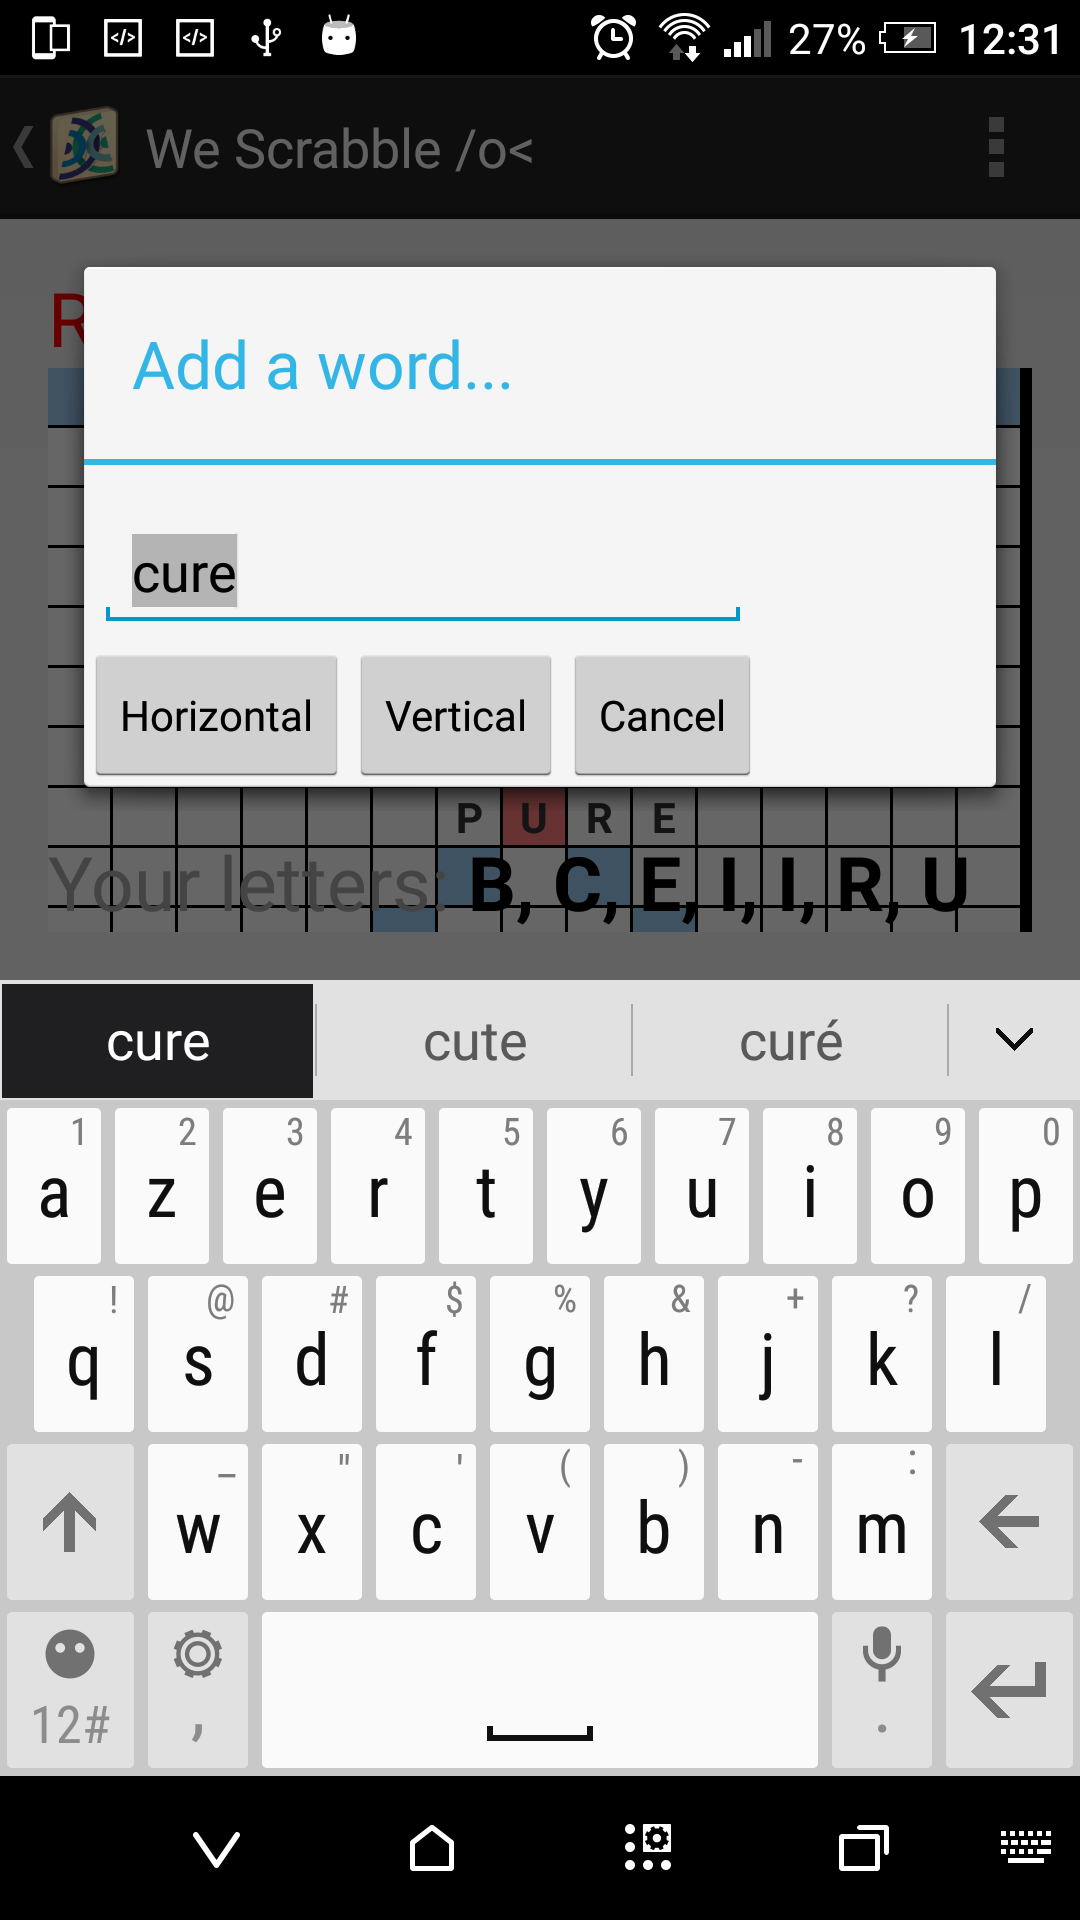
\includegraphics[width=.32\textwidth]{addword.png}
\end{figure}

WeScrabble is a distributed scrabble-like game for Android. When lauching the game, a player first enter its name and choose one of the two teams: red or blue.
When joining the game, he automatically gives 15 letters to its team. Then, he picks 7 letters, with which he can form words to be placed on a grid. In order for a word to be placed on the grid, it must be an existing word, it should fit on the grid, and if it crosses other words the letters should match. The player then pick new letters from its team to have 7 letters on its rack, or until the team has no more letter.

\subsection{Special cells}
\begin{figure}[H]
  \center
  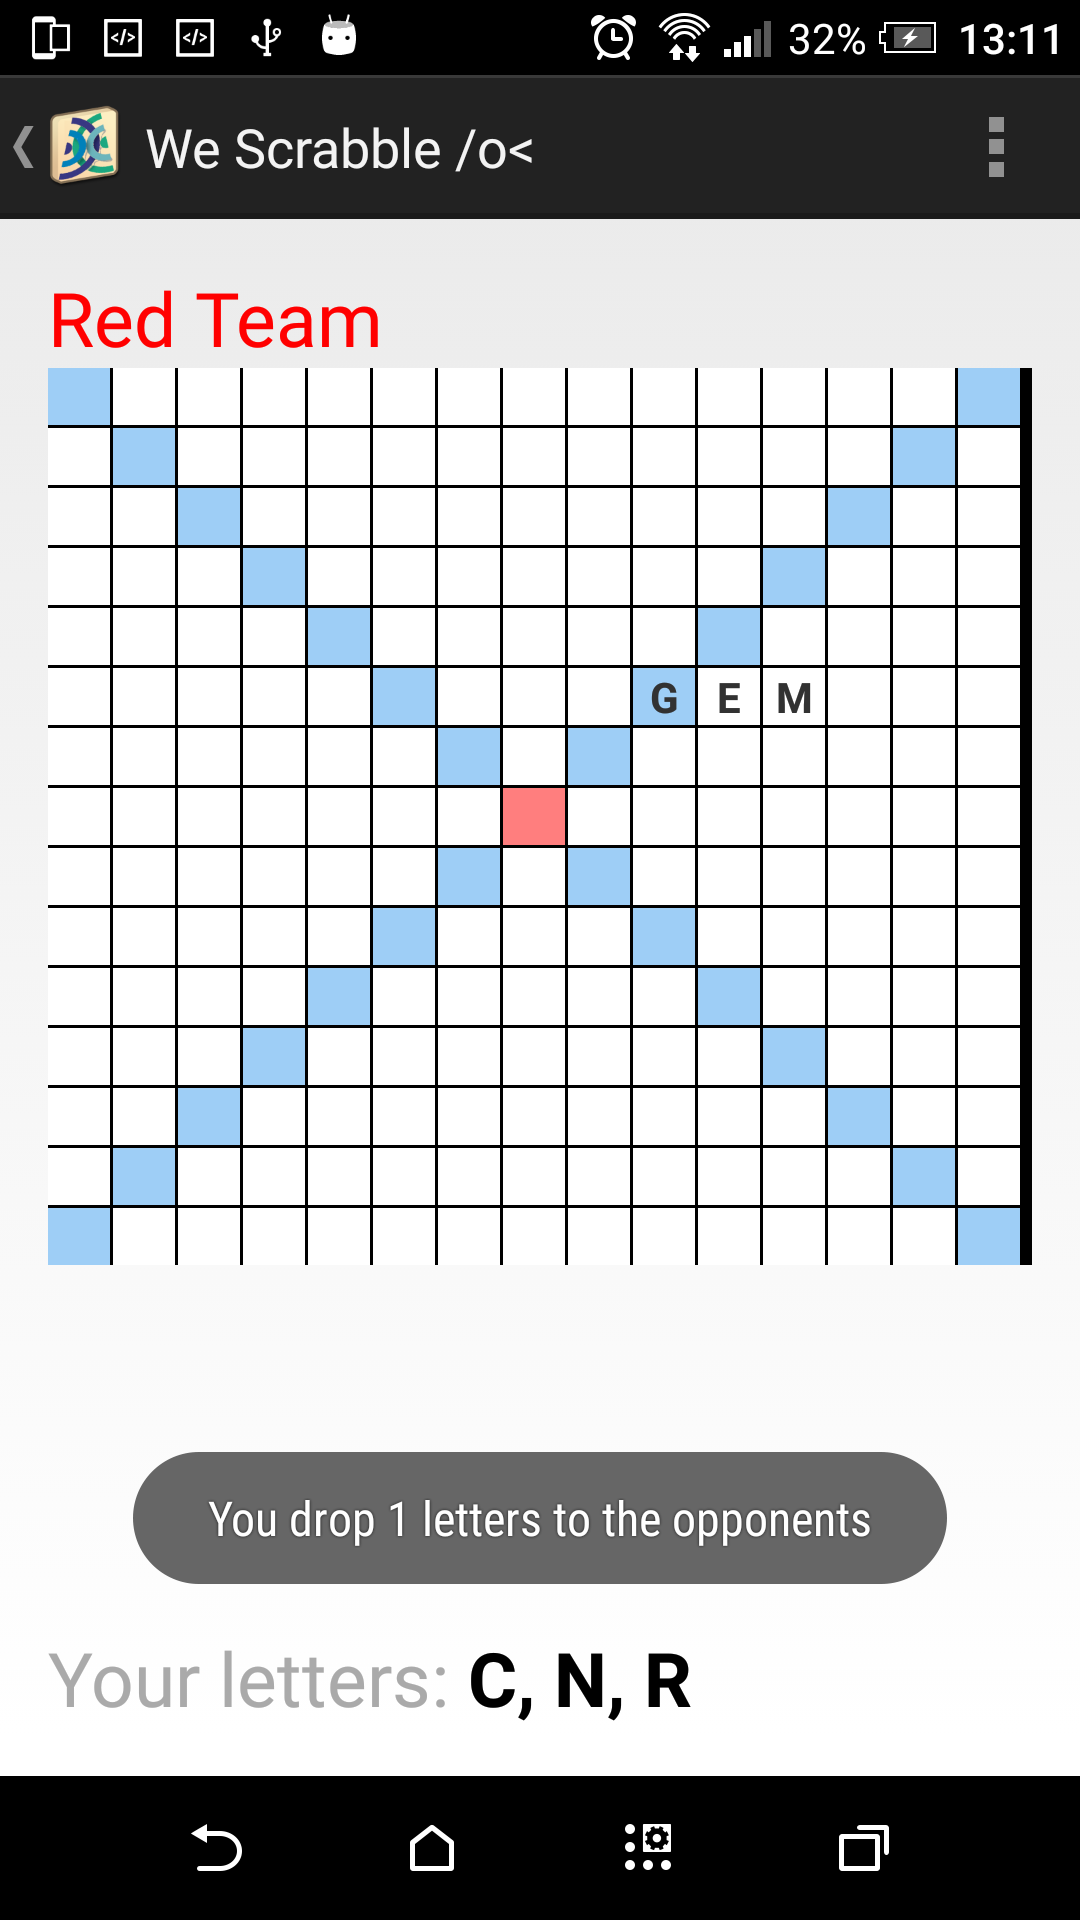
\includegraphics[width=.3\textwidth]{dropletter.png}
\end{figure}

The grid also contains special cells: if a word is placed on the red one, the opponent team gets all the letters of the new word added to its set of letters to be played. If a word is placed on one of the blue cells, the letter on the blue cell is dropped to the opponent team. If a crossing word is added on a special cell, the \textit{attack} also occurs.

\subsection{Exchanging letters}
\begin{figure}[H]
  \center
  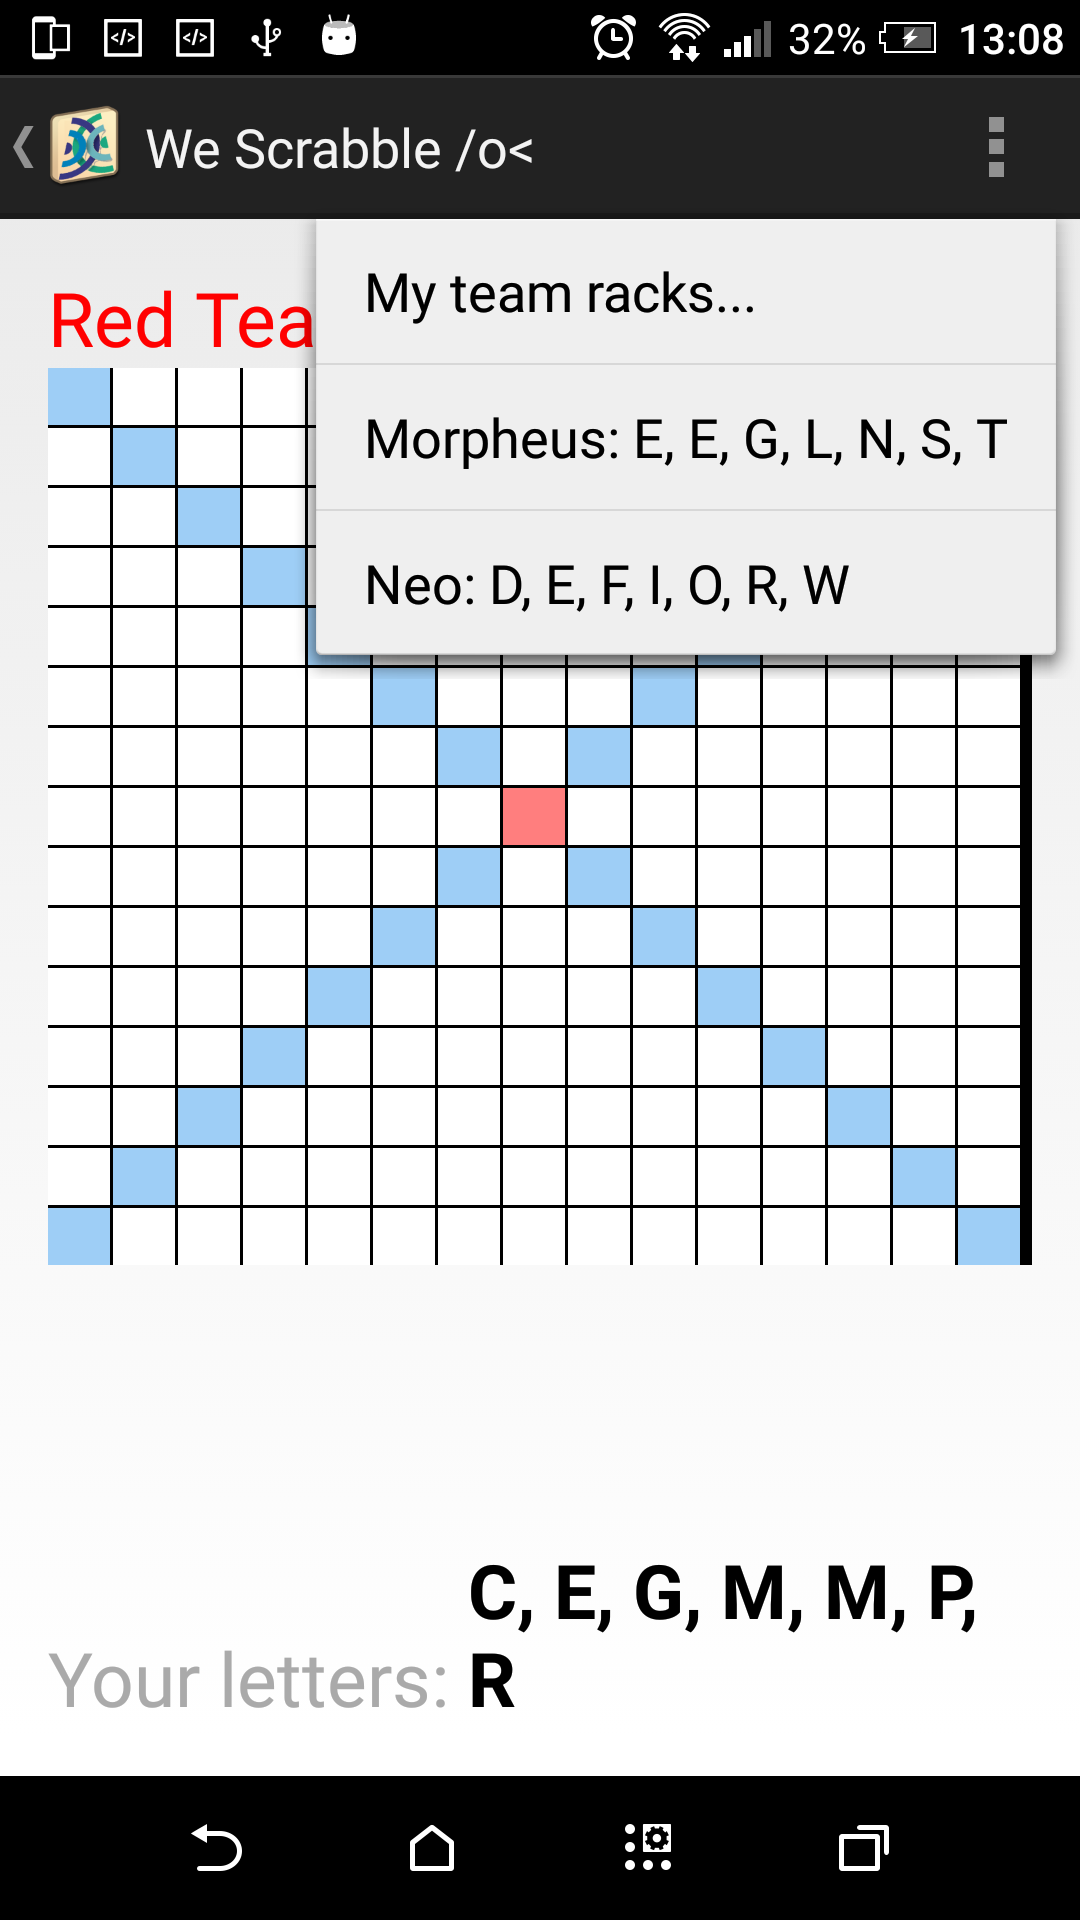
\includegraphics[width=.3\textwidth]{swapletter.png}\hfill
  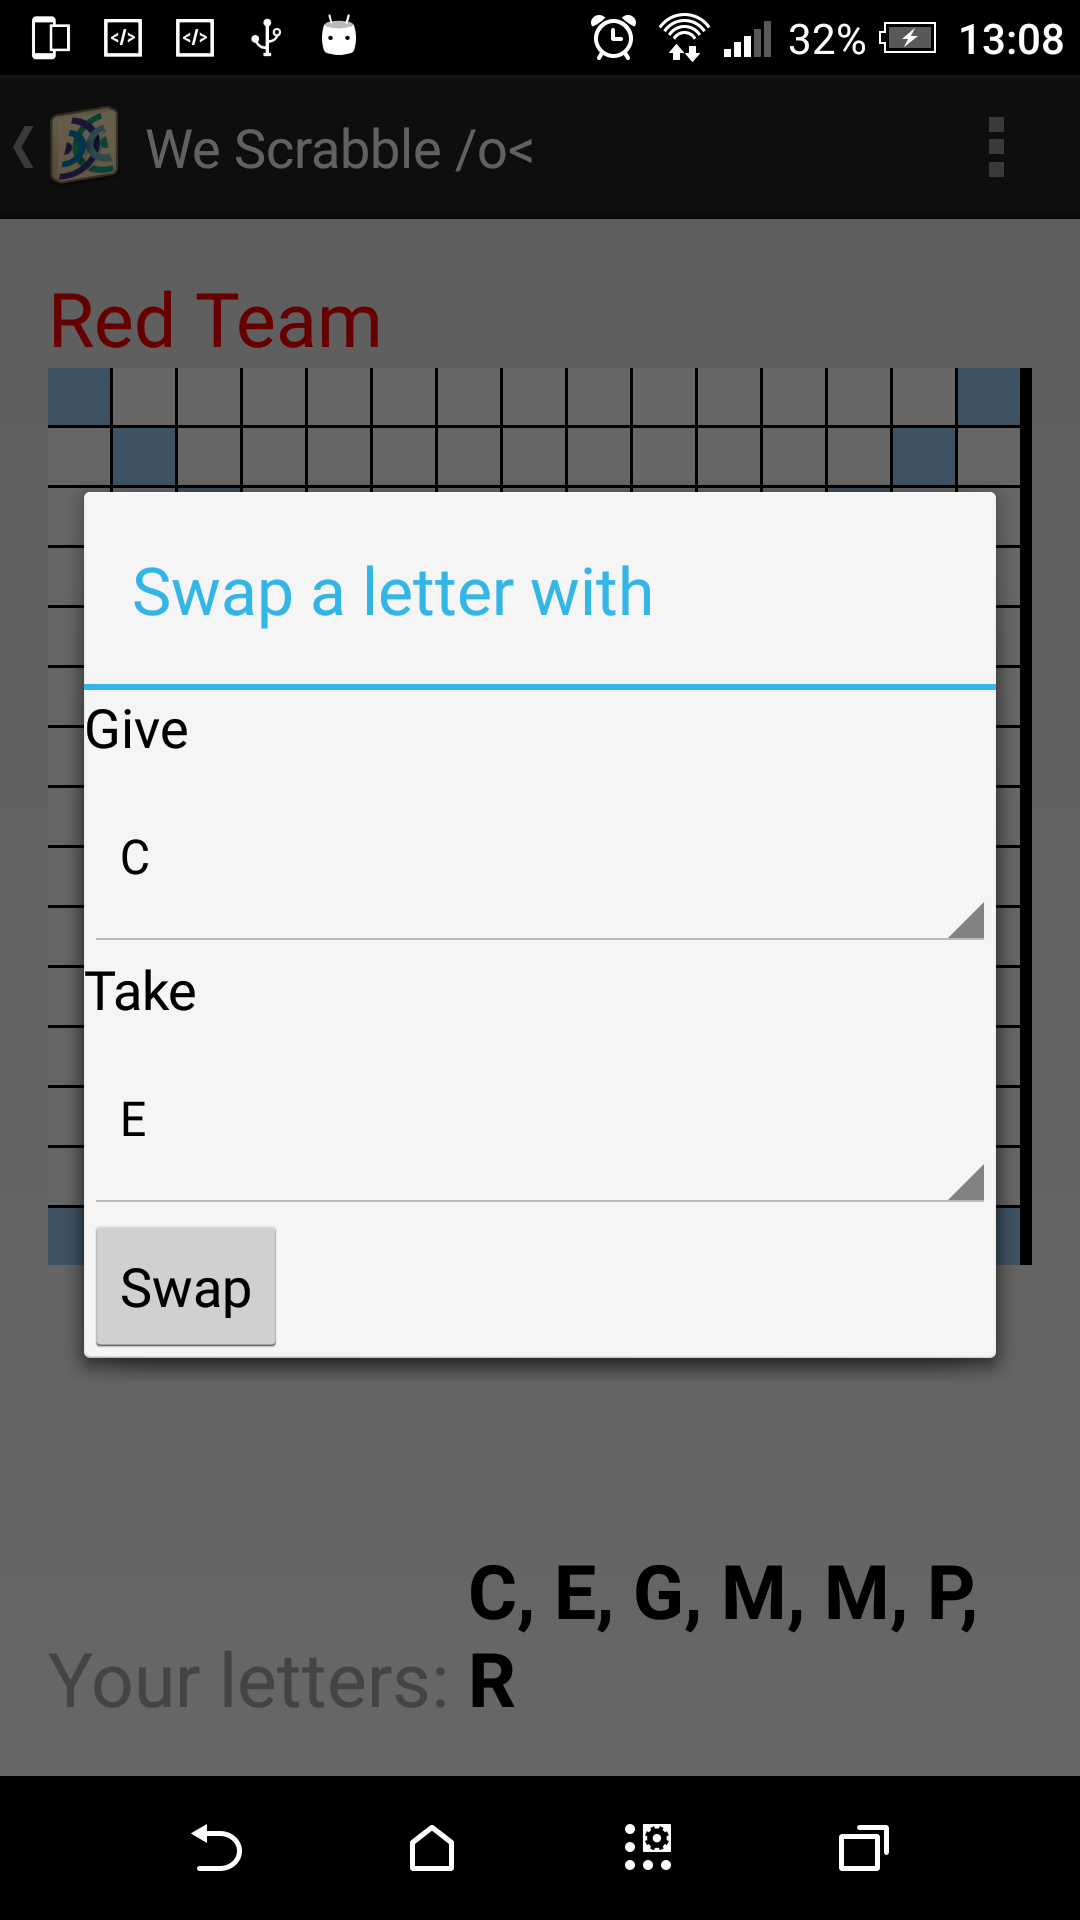
\includegraphics[width=.3\textwidth]{swapletter_dialog.png}
\end{figure}

Players of the same team could also see each other's letters. Two players of the same team can swap letters with each other.

\section{Design choices}
\subsection{Two teams}
The assignment did not state how many teams should be supported. I choosed to only implement 2 teams, because testing on more team, with a limited number of Android devices would have been painful.


\section{Implementation}
\subsection{Foreword}
The very fiust implementation of the game has been realized using ambient references. However, the resulting code was getting more and more complex with the increasing number of features. Th main problem was that time decoupling had to be handled in the application code.

In order to get time decoupling, I then switched to a tuplespace based implementation. All the code had been refactored to use the totam library. However the first tests showed that totam could be very slow, especially on Android. After some frustrating debug time, I decided to implement my own tuplespace system: TamTam.

\subsection{TamTam}
TamTam is a shared tuplespace system, with a single hop replication. Incoming tuples from other tuplespace may be filtered with a user provided function, in order to ignore uninteresting tuples and reduce cache size.

\begin{figure}[H]
  \center
  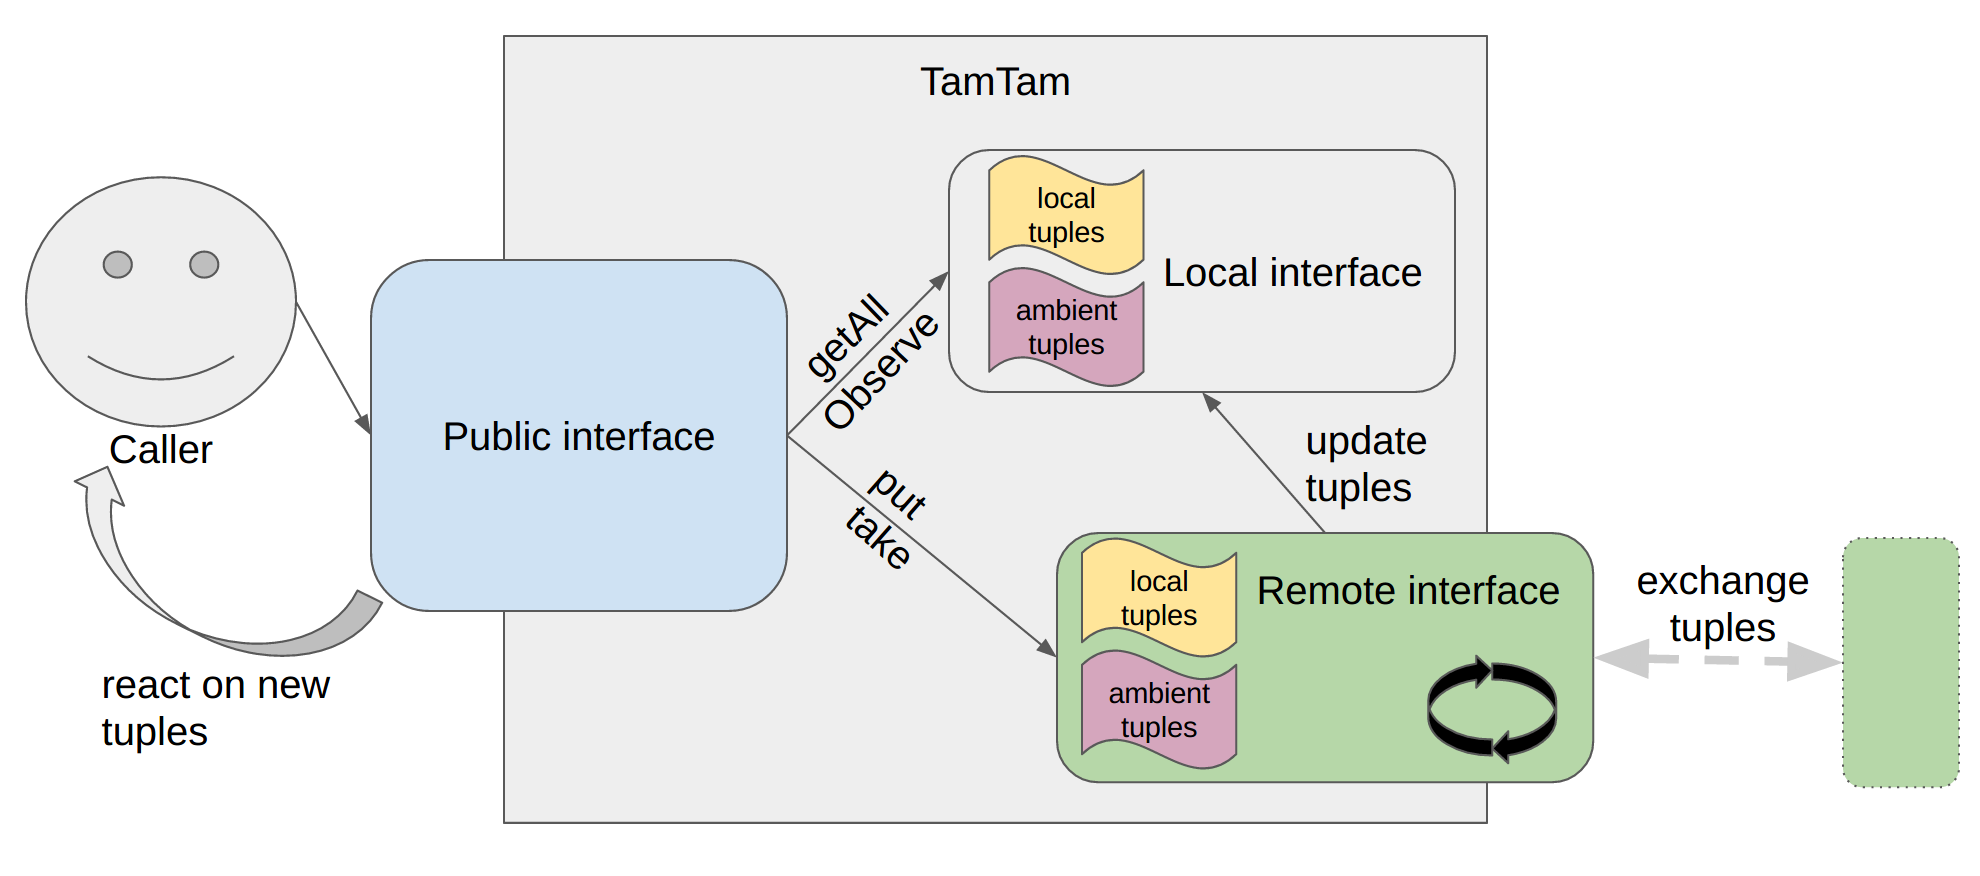
\includegraphics[width=\textwidth]{tamtam.png}
\end{figure}

\subsubsection{Networking actor}
TamTam tuplespaces have an internal actor that performs all communications asynchronously. When a tuple is inserted, it is added to a local database, then propagated to all discovered TamTams. When an ambient tuple is received, it is cached in another database, indexed by discovered peers. When a new TamTam is discovered, the producer sent its whole local database to it.

\subsubsection{Removal}
To remove a tuple, the TamTam on which the removal happens (say the \textit{consumer}) first tries to contact the TamTam that created the tuple (if not himself), the \textit{producer}. Then the consumer deletes the copied tuple from its local cache and resolve a future for the caller. The producer then broadcast the removal of its tuple to all his peers so that their local cache is up to date. This protocol ensure consistency across TamTams, but has the disadvantage that offline tuples could not be taken (like in totam).

\subsubsection{Local interface}
A TamTam also contains a copy of the actor database in order to allow synchronous query of the tuples. When the actor updates its database, it also updates the local interface database.

\subsubsection{Tuple shadowing}
The networking actor also maintains a table of online peers (also replicated in the local interface). When a peer is marked as offline, either with the \texttt{when: ... disconnected: \{...\}} AmbientTalk construct, or when a remote call timeouts, its tuple are shadowed. It means that a query that would match one of the shadowed tuples do not include it in the results. When a disconnected peer is back online, the producer sends a fresh copy of its whole local database so that the consumer is up to date as early as possible.

\subsubsection{Public interface}
\begin{itemize}
  \item \texttt{put(tuple)}: inserts a tuple in the tuplespace
  \item \texttt{getAll(tuple := nil)}: returns all matching tuples known by TamTam when the call has been issued. If no tuple is passed as argument, return all tuples.
  \item \texttt{take(tuple)}: remove a matching tuple from the tuplespace. Return a future that resolves when the deletion completed.
  \item \texttt{observe: tuple do: \{|t|\}}: any time a matching tuple is added, call the given closure with the tuple as argument.
\end{itemize}

\subsection{Tuples}
All tuples exchanged in WeScrabble always have the format $\tau(<Type>, <Team>, ...)$, where Type and Team are AmbientTalk typetags.
\begin{itemize}
  \item $\tau(Player, Team, name:string)$ A player announce itself in a team
  \item $\tau(Letter, Team, letter:string)$ A letter belonging to a team
  \item $\tau(Letter, Team, player:string, letter:string)$ A player takes a letter in its rack.
  \item $\tau(Word, Team, Suggestion)$ A word is added on the grid. The Suggestion is an isolate that contains all the necessary fields to place the word on the grid.
\end{itemize}

\subsection{Random letters}
When a player joins a team and contribute letters to the team letter set, it pick random letters. In order to obtain fairly fair racks of letters, I computed the relative frequency of each letter in the provided dictionary. To pick a random letter, we choose an uniformely distributed real number $q$ between 0 and 1, and return the first $i^{th}$ letter so that $\sum_{k=0}^{i} Freq(i) \geq q$. Therefore, the distribution of letters in the rack should be roughly the same as the distribution of letters in the dictionary.


\section{Improvements}
I really enjoyed working on this project, however due to limited time, I have not implemented all the features I wanted to. In this section I will present a few ones, with a description of how it could be implemented

\subsection{Automatic team}
On the login screen, the user should be able to click a button to automatically choose a team. By couting the number of player tuples in each team, we could assign the player to the team with the least members.

\subsection{Name conflict}
The actual implementation expects the player names to be different, but does not ensure that this is always true. Before joining the game, it might be worth checking if someone else has the same name, and therefore ask the user to provide another name.

\subsection{Fair racks}
For now the program does not fully ensure that the picked up letters are fair. For instance if a player only receives consonants, he will be disadvantaged as it will be more difficult for him to form words. The program could check whether a rack is fair and if not throw away the whole rack to the team pool and pick new letters.

\end{document}
